\chapter{A metodológia alkalmazása a termékfejlesztési folyamatokra}

A \emph{Common Criteria} széleskörű követelményrendszerét olvasva könnyedén a bőség zavarával
küzdhetünk a megfelelő kezdési pont kiválasztásakor. Ez a fejezet azokat a komponenseket szedte egy
csokorba, amelyek a termékfejlesztési folyamatokhoz kapcsolódnak, méghozzá abban a sorrendben, ahogy
az a termékfejlesztés életciklusában előfordul.

\section{Felfedezett hibák vizsgálata biztonsági szempontból (ALC\_FLR)}

Az alábbi szekció a karbantartási folyamat azon részével foglalkozik, miszerint a felfedezett
hibákat (különös tekintettel a biztonsági kockázatot hordozó hibákra) hogyan is kezeljük. A kezelés
fogalmát jelenleg nem tudjuk pontosan meghatározni, ennek feloldása az egyes szinteken lesz
szükséges. A jelenlegi termékfejlesztési folyamatok kezelik a biztonsági hibákat, viszont nincsenek
olyan védőhálók, amelyek az ilyen problémákat mindig szem előtt tartják.

A kiértékelési komponens (ALC\_FLR osztály) szintezésére igaz, hogy a magasabb szinteken
szigorúbbak a hibakezelési folyamatok, és az irányelvek.

\subsection{ALC\_FLR.1 - Basic flaw remediation}
\begin{quote}
    \begin{description}
        \item[ALC\_FLR.1.1D]{The developer shall document and provide flaw remediation procedures
            addressed to TOE developers.}
        \item[ALC\_FLR.1.1C]{The flaw remediation procedures documentation shall describe the
            procedures used to track all reported security flaws in each release of the TOE.}
        \item[ALC\_FLR.1.2C]{The flaw remediation procedures shall require that a description of the
            nature and effect of each security flaw be provided, as well as the status of finding
            a correction to that flaw.}
        \item[ALC\_FLR.1.3C]{The flaw remediation procedures shall require that corrective actions
            be identified for each of the security flaws.}
        \item[ALC\_FLR.1.4C]{The flaw remediation procedures documentation shall describe the
            methods used to provide flaw information, corrections and guidance on corrective actions
            to TOE users.}
    \end{description}
\end{quote}

A \emph{Basic flaw remediation} célja, hogy legyen módszerünk arra, hogy az egyes biztonsági
hibajegyeket és az azokhoz kapcsolódó információkat tudjuk úgy tárolni, hogy az később is
megtalálható legyen, ezáltal elkerülve azt a szerencsétlen eseményt, hogy egy biztonsági résről
egyszerűen elfeledkezünk.

Mivel a hibajegyek kezelésére eleve használunk \emph{JIRA}-t, ezért ha ott felvesszük a ,,biztonsági
rés'' hibajegytípust, és annak kötelező mezőinek megjelöljük a követelmények között listázott
elemeket máris teljesítettük ezt a pontot.

\subsection{ALC\_FLR.2 - Flaw reporting procedures}
\begin{quote}
    \begin{description}
        \item[ALC\_FLR.2.2D]{The developer shall establish a procedure for accepting and acting upon
            all reports of security flaws and requests for corrections to those flaws.}
        \item[ALC\_FLR.2.3D]{The developer shall provide flaw remediation guidance addressed to TOE
            users.}
        \item[ALC\_FLR.2.5C]{The flaw remediation procedures shall describe a means by which the
            developer receives from TOE users reports and enquiries of suspected security flaws in
            the TOE.}
        \item[ALC\_FLR.2.6C]{The procedures for processing reported security flaws shall ensure that
            any reported flaws are remediated and the remediation procedures issued to TOE users.}
        \item[ALC\_FLR.2.7C]{The procedures for processing reported security flaws shall provide
            safeguards that any corrections to these security flaws do not introduce any new flaws.}
        \item[ALC\_FLR.2.8C]{The flaw remediation guidance shall describe a means by which TOE users
            report to the developer any suspected security flaws in the TOE.}
    \end{description}
\end{quote}

A \emph{Flaw reporting procedures} célja röviden, hogy lehetővé tegye a \emph{TOE} felhasználói
számára, hogy biztonsági hibákat jelenthessenek be, és a fejlesztő és a bejelentő felhasználó
között az információáramlás gördülékenyen történjen.

Esetünkben a legegyszerűbb megoldás az lenne, ha a belső \emph{JIRA}-nak lenne egy külső
felhasználók számára elérhető interfésze is (természetesen ekkor figyelembe kell venni a bizalmasabb
információk védelmét). Ekkor a hibajavítás folyamata érdemben nem változik, a szigorúbb követelmény
nem hordoz lényeges nehézséget, csupán a JIRA használatát kell leírnunk úgy, hogy egy tetszőleges
felhasználó is gond nélkül megérthesse.

A \emph{ALC\_FLR.2.7C} pontja szerint meg kell akadályoznunk, hogy a javítás során nem hozunk létre
új biztonsági réseket. Habár a teljesen új rések ellen nem tudunk teljes mértékben védekezni, hiszen
akkor azt a rendes fejlesztésre alkalmazva teljesen meg tudnánk akadályozni azok létrejöttét.
Közelítésként védőhálóinkat úgy határoznám meg, hogy legyen a javításokkor fokozott szakmai
lektorálás, hozzunk létre automatikus teszteseteket a régebbi hibákra regressziós hibák elkerülése
érdekében, és fokozzuk az olyan programok automatikus használatát, amelyek potenciális
sérülékenységeket fedhetnek fel, mint a \emph{fuzzer}ek (például: \emph{American fuzzy lop}),
statikus kódanalizálók.

\subsection{ALC\_FLR.3 - Systematic flaw remediation}

Az előző szinthez képes az alábbi szempontok adódtak hozzá a jelenlegi szinthez:
\begin{quote}
    \begin{description}
        \item[ALC\_FLR.3.6C]{The flaw remediation procedures shall include a procedure requiring
            timely response and the automatic distribution of security flaw reports and the
            associated corrections to registered users who might be affected by the security flaw.}
        \item[ALC\_FLR.3.10C]{The flaw remediation guidance shall describe a means by which TOE
            users may register with the developer, to be eligible to receive security flaw reports
            and corrections.}
        \item[ALC\_FLR.3.11C]{The flaw remediation guidance shall identify the specific points of
            contact for all reports and enquiries about security issues involving the TOE.}
    \end{description}
\end{quote}
Célja annyiban bővül a \emph{Systematic flaw remediation}-nek, hogy a felhasználó számára
biztosított információk között szerepelnie kell annak is, hogy hogyan tudja önmagát regisztrálni
a felhasználó annak érdekében, hogy a biztonsági javítások kiadásáról rövid idő alatt értesítést
kapjon.

Amennyiben elfogadjuk a JIRA-t, mint külső és belső hibajegykezelő eszköz, ennek a megvalósítása
egyszerű, hiszen már beépített funkcionalitás az, hogy lehessen figyelni egy hibajegyet.




\section{Fejlesztési- és karbantartási folyamatok (ALC\_LCD)}
Ez a szekció megmutatja, hogy a jelenlegi, gyengén irányított munkafolyamatainkat miért lenne
előnyös magasabb szinten felügyelni, és milyen kezdeti lépések lennének megfelelőek ennek elérése
irányában.

A \emph{Common Criteria} szempontjából ez azért fontos kérdés, mivel ekkor a \emph{SFR-ek}
megvalósulása egyáltalán nem garantált, amely nyilvánvalóan elfogadhatatlan, mivel azért (is)
vezettük be a \emph{Common Criteria}-t, hogy a termékünk biztonságosabb legyen.

A folyamat gyakorlati alkalmazásának egy lényeges követelménye, hogy a fejlesztést ne akadályozza
számottevően, mivel ilyenkor fennáll a motiváció, hogy ezeket valamilyen módon megkerüljük. Ezzel
ekvivalens követelmény, ha valamilyen módon minimalizáljuk a fejlesztő adminisztrációval eltöltött
idejét, amelyből következik, hogy olyan adminisztrációs eszközt használunk, amely nagyfokú
automatizálást tesz lehetővé, és a nehezen automatizálható feladatok elvégzésére egy nagyon egyszerű
felületet biztosít.

\subsection{Jelenleg használt munkafolyamataink}
A jelenlegi munkafolyamatokat \aref{fig:oldfeature} és \aref{fig:oldmt} ábrán található gráfok
jellemzik, ahol az egyes csomópontok a fentebb említett állapotok közül lehetségesek, az élek pedig
az engedélyezett átmeneteket jelentik.

\begin{figure}[h]
    \centering
    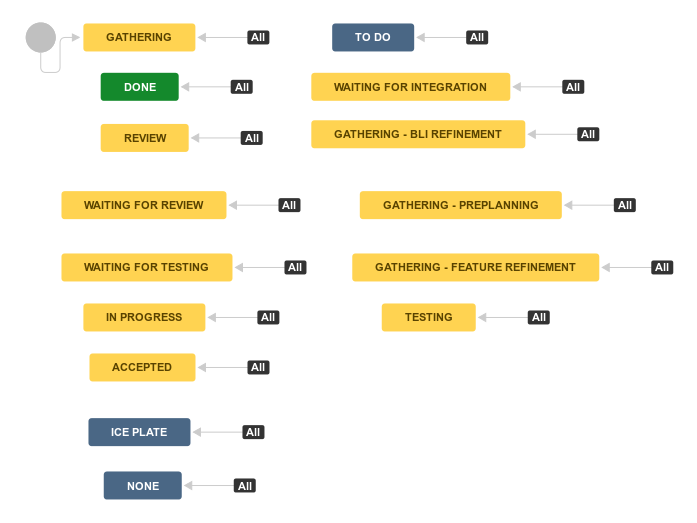
\includegraphics[width=\textwidth, height=0.4\textheight, keepaspectratio]{figures/oldfeature.png}
    \caption{A \emph{syslog-ng} fejlesztéséhez jelenleg használt, megengedő folyamat}
    \label{fig:oldfeature}
\end{figure}
\FloatBarrier
\pagebreak[3]

\begin{figure}[h]
    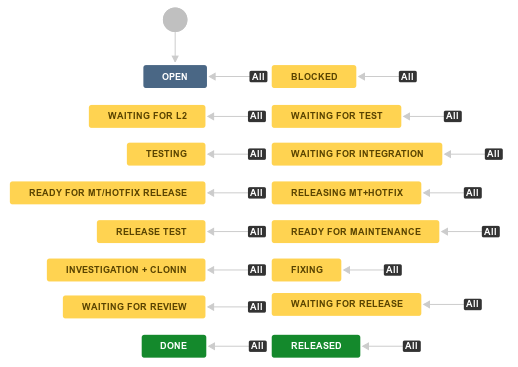
\includegraphics[width=\textwidth, height=0.4\textheight, keepaspectratio]{figures/oldmt.png}
    \centering
    \caption{A \emph{syslog-ng} karbantartásához jelenleg használt, megengedő folyamat}
    \label{fig:oldmt}
\end{figure}

\FloatBarrier
\pagebreak[3]
\subsection{Szigorítások a folyamatokon}

Mint ahogy az a gráfokból leolvasható, sajnos tetszőleges két állapot között megengedett átmenet,
ezért például lehetséges egy hiba javításánál a szakmai lektorálás kihagyása, amely jobb esetben
csak a kód minőségének romlásához, legrosszabb esetben viszont kártékony kód kódbázisba kerüléséhez
vezethet.

Első közelítésben érdemes korlátozni a lehetséges átmeneteket. Ennek eredményét
\aref{fig:newfeature} és \aref{fig:newmt} ábrán látható folyamatok mutatják.

\begin{figure}[h]
    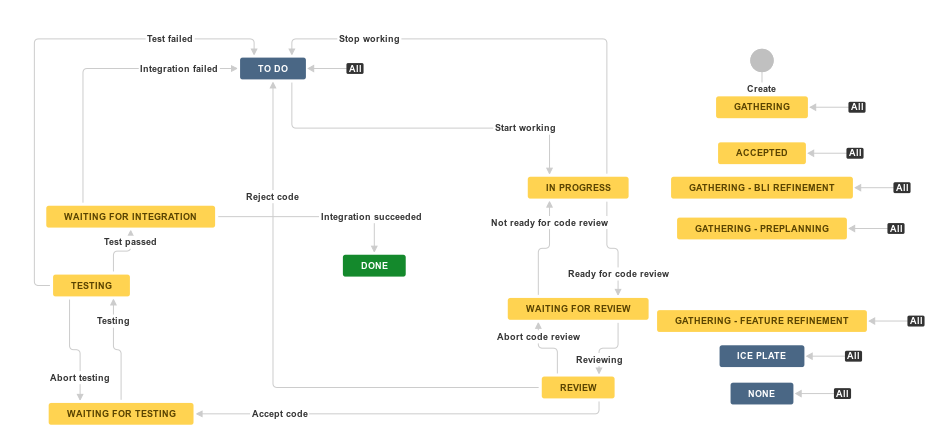
\includegraphics[width=\textwidth, keepaspectratio]{figures/newfeature.png}
    \centering
    \caption{A \emph{syslog-ng} fejlesztéséhez javasolt, szigorított folyamat}
    \label{fig:newfeature}
\end{figure}

\begin{figure}[h]
    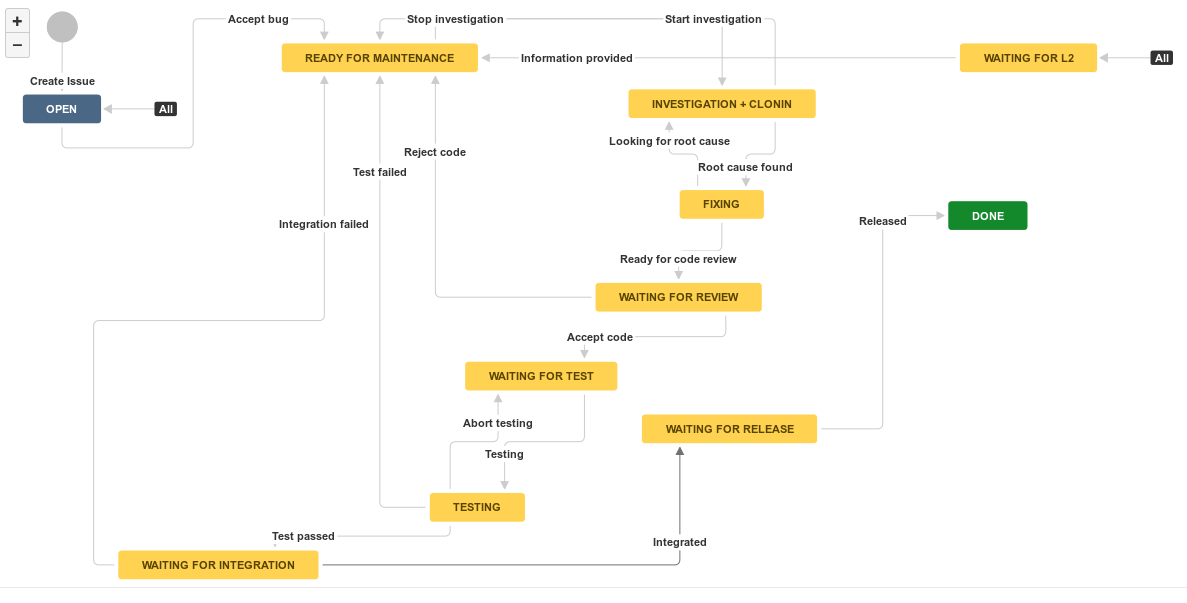
\includegraphics[width=\textwidth, keepaspectratio]{figures/newmt.png}
    \centering
    \caption{A \emph{syslog-ng} karbantartásához javasolt, szigorított folyamat}
    \label{fig:newmt}
\end{figure}

\FloatBarrier

Az átmenetek létrehozásával lehetőségünk nyílt \emph{JIRA}-ban az egyes átmenetekhez
\begin{itemize}
    \item \emph{feltétel}eket (olyan előfeltételek, amelyek teljesülése engedi az állapot
        végrehajtását),
    \item \emph{validator}okat (olyan ellenőrzések, amelyek az átmenet végrehajtása előtt
        értékelődnek ki),
    \item és \emph{post function}-öket (olyan műveletek, amelyek az átmenet végrehajtása után
        lefutnak)
\end{itemize}
definiálni. Ez az eszköztár segíthet abban, hogy ne csupán lassítsuk a kritikus állapotok
átugrásának kísérletét, de akár kényszeríthetjük, hogy más emberekkel együtt kelljen működnie ahhoz,
hogy a szándékolt változtatást végrehajtsa. Feltételezhetjük, hogy a belső támadó számára ez már
elég költséges és/vagy kockázatos ahhoz, hogy inkább más módszert keressen.

Ez például megvalósítható úgy, hogy eltárolom azokat a fejlesztőket, akik létrehozták a megoldást
(azaz azokat, akik valaha ,,\emph{To do}''-ból ,,\emph{In progress}''-be mozgatták az adott jegyet),
és csak annak engedem a tesztelésen és a lektoráláson való továbbengedést, akik nincsenek benne az
előbb létrehozott listában.

További kényelmi funkciókat is megalapoztunk az átmenetek szétválasztásával, mint például azt, hogy
végrehajtásukkor van lehetőségünk a JIRA felhasználótól információt bekérni.  Ez önmagában nem tűnik
nagy előnynek, de ha belegondolunk, akkor például a karbantartás tanulási görbéje kevésbé lett
meredek, hiszen így már nem kell ismerni, globálisan a folyamatot, elegendő lokális döntéseket
meghozni (átment-e a módosítás a teszteken, vagy sem), illetve nem kell ismerni például azt sem,
hogy mielőtt a tesztelőknek odaadnám a módosításaimat, létre kell hoznom egy teljes
telepítőcsomagot, ha a \emph{JIRA} rákérdez az átmenet végrehajtása előtt, hogy milyen elérési
útvonalon találja meg a generált telepítőcsomagot. Ez a megközelítés gyakorlatilag
a \emph{fail-fast} \cite{shore2004fail} szoftverfejlesztési technika folyamatokra vetített
változata.

\pagebreak[3]
\section{Configuration Management}
A \emph{Configuration Management} (továbbiakban: \emph{CM}) egy olyan rendszer, amely arra hivatott,
hogy azokat a változtatásokat nyomon tudja követni, amelyek hatással lehetnek a vizsgált termékre.
Amennyiben csak jól meghatározott, autorizált változtatásokat engedélyezünk, biztosíthatjuk a
termékünk integritását.

\subsection{Configuration Management Scope (ALC\_CMS)}
Természetesen mielőtt egyáltalán bevezetnénk a \emph{CM}-et, szükséges meghatározni annak hatókörét.
Ez a szekció meghatározza azokat a dolgokat, amelyeket feltétlenül szükséges a \emph{CM} rendszerben
kezelnünk, a szinteket is ez határozza meg (azaz magasabb szinten többet kell lefednie
a \emph{CM}-nek).

\pagebreak[3]
\subsubsection{ALC\_CMS.1 - TOE CM coverage}
\begin{quote}
    \begin{description}
        \item[ALC\_CMS.1.1D]{The developer shall provide a configuration list for the TOE.}
        \item[ALC\_CMS.1.1C]{The configuration list shall include the following: the TOE itself; and
            the evaluation evidence required by the SARs.}
        \item[ALC\_CMS.1.2C]{The configuration list shall uniquely identify the configuration
            items.}
    \end{description}
\end{quote}

Ennek a szintnek a létjogosultsága triviális, hiszen a \emph{CM}-nek definíció szerint tartalmaznia
kell a \emph{TOE}-t, hiszen annak integritásának megőrzése a CM elsődleges feladata. Az
\emph{evaluation evidence}-ek követése azért fontos, mivel a követelmények teljesülését be kell
tudni mutatni. Ezeknek a bizonyítékoknak szoros kapcsolatban kell lenniük a TOE-val annak elkerülése
érdekében, hogy olyan szempont teljesülését állítsuk, amely egy régebbi TOE-ban valóban teljesült,
de egy újabb verzióban már nem.

Ez az első elem, amelyet felvettünk a CM-be, ezért eddig csak általánosságban beszéltünk róla, és
nem definiáltuk, hogy konkrétabban milyen rendszerek alkotják a CM-et.  Mivel maga a kész TOE egy
bináris, ezért a követésére egy \emph{binary repository manager}-re (vagy \emph{artifact
repository}-ra) van szükségünk, de ezen a ponton akár felhasználhatjuk azt is, hogy a ZBS valahol
belül rendezetten tárolja az egyes fordítások eredményeit, de egy független repository használata
bölcsebb gondolatnak tűnik.  Az egyedi azonosításhoz használhatjuk a TOE egyedi címkéjét, amelyet az
3.3.2.1-es alszekcióban részletesebben kifejtjük.

\pagebreak[3]
\subsubsection{ALC\_CMS.2 - Parts of the TOE CM coverage}
\begin{quote}
    \begin{description}
        \item[ALC\_CMS.2.1C]{The configuration list shall include the following: [\ldots] \emph{and
            the parts that comprise the TOE}.}
        \item[ALC\_CMS.2.3C]{For each TSF relevant configuration item, the configuration list shall
            indicate the developer of the item.}
    \end{description}
\end{quote}

Ennek a követelménynek a megfogalmazása részben zavaros, ezért az \emph{Application notes} alapján
a TOE részei alatt például az olyan alkalmazásokat kell érteni, amelyeket a felhasználónak is
szállítunk. Esetünkben ilyen maga a \emph{syslog-ng} bináris, de beleértendőek a különböző
debug információkat összegyűjtő eszközök, naplóbejegyzéseket tesztelési céllal előállító
segédprogramok is. Ez a pont általában megvalósul az ALC\_CMS.1-gyel együtt, legalábbis első
közelítéskor egyértelműnek tűnt, hogy ezt is követni kell, mert hatással van a TOE-ra.

Az ALC\_CMS.2.3C-nél a ,,fejlesztőt'' úgy kell érteni, mint fejlesztő szervezetet, nem mint konkrét
személyt. Ennek a teljesülése is természetes szokott lenni, hiszen a dependenciáinkat érdemes
már csak a frissítések miatt is követni, ehhez pedig szükséges tudni azt, hogy ki is fejlesztette.

\pagebreak[3]
\subsubsection{ALC\_CMS.3 - Implementation representation CM coverage}
\begin{quote}
    \begin{description}
        \item[ALC\_CMS.3.1C]{The configuration list shall include the following: [\ldots];
            \emph{and the implementation representation}.}
    \end{description}
\end{quote}

Mint látható, csupán annyit változott a követelmény, hogy az implementációs reprezentációt (, azaz
gyakorlatilag a termék forráskódját) \emph{CM}-ben kezeljük. Mivel már minden forráskódot
a \emph{git} verziókezelővel követünk, ezért ha ezt a rendszert beleértjük a CM-be, akkor könnyedén
teljesíthetjük ezt a követelményt. (Természetesen ez csak azzal a kitétellel igaz, ha a \emph{git}
rendelkezik a megfelelő képességekkel.)

\pagebreak[3]
\subsubsection{ALC\_CMS.4 - Problem tracking CM coverage}
\begin{quote}
    \begin{description}
        \item[ALC\_CMS.4.1C]{The configuration list shall include the following: [\ldots]; \emph{and
            security flaw reports and resolution status}.}
    \end{description}
\end{quote}

A \emph{flaw remediation} részben arra a konklúzióra jutottunk, hogy a biztonsági hibákat
\emph{JIRA}-ban \cite{JIRA} követjük, ezért a \emph{CM} rendszerhez érdemes hozzávennünk magát
a \emph{JIRA}-t is, pontosan úgy, mint ahogy az előző pontban tettük. Mivel azonban már három
független rendszer összekapcsolásánál járunk, egyre jobban kell figyelnünk a megfelelő
szinkronizáció kialakításánál.

\pagebreak[3]
\subsubsection{ALC\_CMS.5 - Development tools CM coverage}
\begin{quote}
    \begin{description}
        \item[ALC\_CMS.5.1C]{The configuration list shall include the following: [\ldots]; security
            flaw reports and resolution status; \emph{and development tools and related
            information}.}
    \end{description}
\end{quote}

A fejlesztői eszközök (olyan eszközök, amelyek részt vesznek a termék létrehozásában) és azok
konfigurációi definíció szerint olyan dolgok, amelyek módosításait \emph{CM} rendszerben erősen
ajánlott követnünk, hiszen ha például lehetőségünk van autorizálatlanul az egyes fordítóprogramokat
tetszőleges binárisra lecserélnünk, máris tetszőlegesen módosíthatjuk a \emph{TOE}-t annak
generálása során, vagy ha ugyan az eszközök változásait követjük, de a konfigurációjáét nem, akkor
például egyes fordítói ellenőrzések kikapcsolásával, olyan hibákat engedhetünk a kódban, amelyeket
már a fordítás során is észrevehettünk volna.

Ezt a követelményt továbbfejleszthetjük úgy, hogy a \emph{Infrastructure as Code, IaC}
\cite{huttermann2012infrastructure} paradigmát szem előtt tartva olyan formában írjuk le, amely
alkalmas a fejlesztési környezet könnyű reprodukciójához. Ilyen például a \emph{syslog-ng}
fordítására alkalmas \emph{Docker} konténert leíró \emph{Dockerfile}. \cite{syslogngenv}

Ennek a követelménynek a betartatásánál könnyedén túlzásokba is eshetünk úgy, hogy azt
a környezetet, amelyben a implementációs reprezentáción dolgozunk, fejlesztőinek tekintjük, és
korlátozzuk a fejlesztőket ennek használatára. Belátható, hogy ez feleslegesen mehet
a termelékenység rovására.

\pagebreak[3]
\subsection{Configuration Management Capabilities (ALC\_CMC)}

A \emph{CM} másik lényeges összetevője annak definiálása, hogy maga a rendszer milyen
változtatásokat engedélyez a felügyelt elemein. Erre szolgál az \emph{ALC\_CMC} alosztály.
Az előző alosztályokhoz hasonlóan a szintek meghatározása az ellenőrzések szigorúságával van
összefüggésben.

\subsubsection{ALC\_CMC.1 - Labelling of the TOE}
\begin{quote}
    \begin{description}
        \item[ALC\_CMC.1.1D]{The developer shall provide the TOE and a reference for the TOE.}
        \item[ALC\_CMC.1.1C]{The TOE shall be labelled with its unique reference.}
    \end{description}
\end{quote}

Az \emph{EAL1} szint elérése ennél az alosztálynál egy egészen egyszerű feladatnak tűnik, hiszen
csupán annyi a feladat, hogy a termék egy adott állapotát egy egyedi címkével ellássuk, és mivel
a verziószám készítése manapság elterjedt, ezért adódik, hogy legyen ez az egyedi címkénk.

Sajnos ez csak addig ennyire egyszerű, amíg nem jutunk el a kiadás létrehozásáig: vannak olyan
teszteseteink (továbbiakban: \emph{Release teszt}), amelyek futtatása költséges, és/vagy különleges
eszközökön kell azt futtatni. Ezt korábban úgy oldottuk fel, hogy az ilyen tesztek futtatását
a kiadás létrehozásáig elodáztuk.  Amennyiben anomáliát észlelünk, a javítástól újraindítjuk
a termékfejlesztés folyamatát, és \emph{a címkét átmozgatjuk a javított állapotra}, amellyel azonnal
megsérthetjük a címkék egyediségének feltételét , ha az átmozgatás nem mindenütt történik meg,
továbbá ez a fejlesztők között is könnyedén félreértésekhez vezethet.

Adódik a javaslat is, hogy külön jelöljük azokat a verziókat, amelyek eljutottak a Release tesztig,
például a széles körben használt \emph{sorszámozott Release Candidate}, röviden \emph{rc}
szuffixszel.
Alternatív módszerek lehetnek az alábbiak:
\begin{itemize}
    \item \emph{git describe} használata: \\
        Például: \emph{syslog-ng-3.7.2-834-gdb3795a}, amely az alábbi formátumnak felel meg: \\
        \emph{<commit-tól a szülők felé lépdelve az első elérhető tag>-<az elért tagtől hány commit
            történt a paraméterben kapott commit-ig>-<verziókezelőt leíró karakter><paraméterben
        átadott commit commitid-ja>}
    \item előfordulhat, hogy nem tekinthetjük a \emph{git}-et függőségnek, ilyenkor
        a \emph{commitid} létrehozásához hasonlóan generálhatunk egy \emph{hash}-t
        a \emph{configuration item}-ből, amely ugyan nem garantáltan egyedi, de jó hash függvény
        esetén az ütközés esélye elhanyagolható.
\end{itemize}

\pagebreak[3]
\subsubsection{ALC\_CMC.2 - Use of a CM system}

\begin{quote}
    \begin{description}
        \item[ALC\_CMC.2.2D]{The developer shall provide the CM documentation.}
        \item[ALC\_CMC.2.3D]{The developer shall use a CM system.}
        \item[ALC\_CMC.2.2C]{The CM documentation shall describe the method used to uniquely
            identify the configuration items.}
        \item[ALC\_CMC.2.3C]{The CM system shall uniquely identify all configuration items.}
    \end{description}
\end{quote}
Látszatra ennek a követelménynek nem sok jelentősége van, hiszen egy olyan rendszert használnánk,
amely egyelőre nem követel meg semmit, csupán azt, hogy a követett elemei legyenek egyedileg
azonosíthatóak. Ennek a pontnak sokkal inkább az a motivációja, hogy a komponensekre osztott TOE
kezelését megalapozzuk.

\pagebreak[1]
\subsubsection{ALC\_CMC.3 - Authorisation controls}
\begin{quote}
    \begin{description}
        \item[ALC\_CMC.3.4C]{The CM system shall provide measures such that only authorised changes
            are made to the configuration items.}
        \item[ALC\_CMC.3.5C]{The CM documentation shall include a CM plan.}
        \item[ALC\_CMC.3.6C]{The CM plan shall describe how the CM system is used for the
            development of the TOE.}
        \item[ALC\_CMC.3.7C]{The evidence shall demonstrate that all configuration items are being
            maintained under the CM system.}
        \item[ALC\_CMC.3.8C]{The evidence shall demonstrate that the CM system is being operated in
            accordance with the CM plan.}
    \end{description}
\end{quote}

Ez az a pont, ahol a \emph{CM} használata értelmet nyer, mivel innentől már nem engedélyez
tetszőleges módosításokat a kódbázison, ezáltal csökkentve a lehetőségét a \emph{TOE} rosszindulatú
módosításának.

Mivel előző pontban beláttuk a \emph{git} \emph{CM}-ként való  használatának előnyét, és
a \emph{git}-et elsődlegesen forráskódok kezelésére használják, ezért visszavezethetjük
a problémánkat arra, hogy hogyan \emph{szokás} a forráskód módosításainál eldönteni, hogy az
autorizált-e.  Észrevehetjük, hogy a nyílt, közösség által fejleszett projektek ezt meg tudják úgy
oldani, hogy:
\begin{itemize}
    \item{csak olyan változtatások kerülhetnek be a kódbázisba, amelyet egy szűkebb csoport
        elfogad,}
    \item{mégsem szűkül a lehetséges kontribútorok halmaza, azaz gyakorlatilag bárki
        kontributálhat.}
\end{itemize}

Ezen feltételek egy lehetséges megoldása az úgynevezett \emph{Forking Workflow}-t használata
a fejlesztésre, amely röviden az alábbi lépésekből áll:
\begin{enumerate}
    \item{Létrejön egy ún. \emph{blessed repository}, amely a forráskód referenciaváltozatát
        tartalmazza.}
    \item{Az egyes fejlesztők leklónozzák ezt a \emph{repository}-t sajátként (ez a művelet úgy is
        ismert, mint \emph{fork}olás)}
    \item{A fejlesztő a saját \emph{repository}-jában elkészíti a módosításait.}
    \item{Valamilyen módon értesíti a \emph{blessed repository} tulajdonosát
        (nevezzük ezt a személyt \emph{integrátornak}) az elkészített változtatásokról.}
    \item{Az integrátor elfogadja, vagy elveti a javasolt változtatásokat.}
\end{enumerate}

\begin{figure}[h]
    \centering
    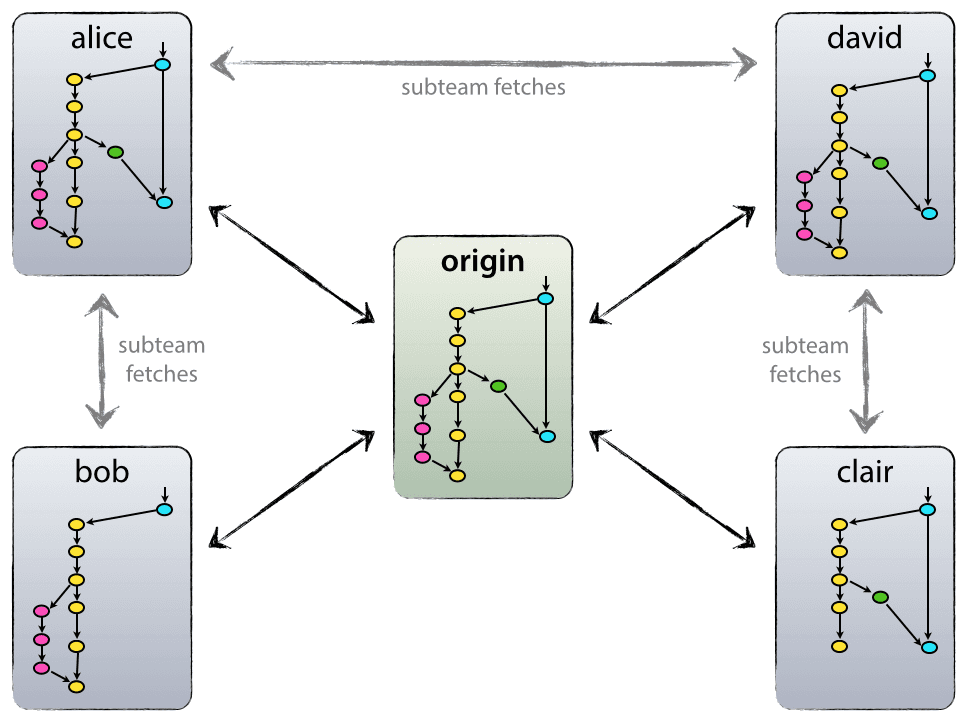
\includegraphics[width=\textwidth, height=0.25\textheight,
    keepaspectratio]{figures/forkingworkflow.png}
    \caption{Példa az egyes kontribútorok és a \emph{blessed repository} viszonyáról
    \cite{driessen2010successful}.}
\end{figure}
\FloatBarrier

Természetesen ahhoz, hogy ez működjön, meg kell tiltani a \emph{blessed repository} írását a többi
fejlesztő által(, vagy legalábbis csak kivételes esetekben szabad ezeket engedélyezni).

A \emph{syslog-ng}-nél a közösség által fejlesztett változatban már korábban igazodni kellett ehhez
a munkafolyamathoz, a kereskedelmi célú változatában ezt a gondolkodásmódot még erősíteni szükséges,
mivel általában a módosítások integrálásának kérelme (továbbiakban: \emph{pull/merge request}) meg
szokott történni, de ez a \emph{blessed repository} egyik ágának a másikára szokott történni, azaz
semmi sem garantálja, hogy egy fejlesztő ne csak az általa létrehozott \emph{branch}-et tudja írni.

\pagebreak[1]
\subsubsection{ALC\_CMC.4 - Production support, acceptance procedures and automation }
\begin{quote}
    \begin{description}
        \item[ALC\_CMC.4.4C]{The CM system shall provide \emph{automated} measures such that only
            authorised changes are made to the configuration items.}
        \item[ALC\_CMC.4.5C]{The CM system shall support the production of the TOE by automated
            means.}
        \item[ALC\_CMC.4.8C]{The CM plan shall describe the procedures used to accept modified or
            newly created configuration items as part of the TOE.}
    \end{description}
\end{quote}

Azaz ez a szekció a magasabb szintű automatizálás megvalósítására hivatott, mivel az
alapfeltételezés az, hogy az emberi tényező megbízhatósága lényegesen alacsonyabb lehet egy
megegyező munkát végző géppel, főként az amúgy könnyedén automatizálható feladatoknál.  Mint ahogy
az a követelményekből látszik, a \emph{Common Criteria} csak az autorizált változtatások bekerülését
szabályozná automatikusan, viszont érdemes továbbgondolni a feladatot, mivel ha az \emph{4.8C}-ben
említett pontot kellőképpen formálisan írjuk le, akkor abból könnyedén programkód készülhet, és
végsősoron az ellenőrzések egy részhalmazát automatikusan megtehetjük.  Az alosztály továbbá
megköveteli a TOE automatikus létrehozhatóságát is. Ez összhangban áll a \emph{Continuous
Integration}\cite{fowler2006continuous} használatával.

A \emph{syslog-ng} közösség által fejlesztett változatánál a legnagyobb elmaradás az elfogadás
szükséges feltételeinek dokumentálása, és az automatizálható ellenőrzések automatizálása.

Van az ellenőrzéseknek egy olyan fajtája, amelyeket csak az újonnan beérkező kódra szeretnénk
alkalmazni, mint például a kódstílus egységesítése automatikus formázók segítségével: mind annak
azonnali alkalmazása, mind a stílusleíró változásával járó újraalkalmazás túl nagy különbséget
eredeményezne a formázás előtti és utáni kód között (ha például a jelenlegi \emph{master} ágon
szeretném az összes \emph{C} nyelven írt forrásfájlt formázni, akkor az önmagában egy $16375$ sor
hozzáadásával és $15982$ sor törlésével járna). Ennek teljes körű szakmai lektorálása nehézkes az
átnézendő kód mérete miatt, a lektorálatlan kódról pedig feltételeznünk kell, hogy kártékony
módosításokat tartalmazhat, hiszen az esetek nagy részében a \emph{syslog-ng} \emph{root}
felhasználóként fut, akinek a jogköre már egészen széles szokott lenni ahhoz, hogy érdemes legyen
megszemélyesíteni.

Az ilyen transzformációk miatt felmerült egy olyan könnyűsúlyú (ezáltal CI rendszerbe integrálható)
eszköz létrehozása, amely képes ellenőrzéseket és átalakításokat végrehajtani csak és kizárólag
néhány kódmódosítási egységen (pontosabban az adott verziókezelő által atominak tekintett
módosításokon, más néven \emph{commit}-okon), míg a kódbázis maradékát érintetlenül hagyja.
Ellenőrzések esetén így megtalálhatjuk az első olyan \emph{commit}-ot, amely egy adott szempontból
nem megfelelő, transzformációk esetén pedig \emph{commit}-ról \emph{commit}-ra tehetünk javaslatokat
a javításra.

Fontos megjegyezni, hogy az eszköz hatékony használatához elengedhetetlen a \emph{commit}-ok
jólszervezettsége, hiszen minél kisebb egy módosítás, annál könnyebb a problémáit észrevenni,
illetve ellenőrizni, hogy az eszközeink úgy módosították a kódot, ahogy azt elvártuk.

Amint a lektorok elfogadták a módosítási javaslatot, és az egyes ellenőrzések sem találtak
kivetnivalót benne, elfogadhatónak tekinthető az, és akár az ellenőrzést végző \emph{CI} rendszer
automatikusan el is fogadhatja, amellyel az \emph{ALC\_CMC.4.4C} pontját teljesítettük.

\subsubsection{ALC\_CMC.5 - Advanced support}
\begin{quote}
    \begin{description}
        \item[ALC\_CMC.5.3C]{The CM documentation shall justify that the acceptance procedures
            provide for an adequate and appropriate review of changes to all configuration items.}
        \item[ALC\_CMC.5.7C]{The CM system shall ensure that the person responsible for accepting a
            configuration item into CM is not the person who developed it.}
        \item[ALC\_CMC.5.8C]{The CM system shall identify the configuration items that comprise the
            TSF.}
        \item[ALC\_CMC.5.9C]{The CM system shall support the audit of all changes to the TOE by
            automated means, including the originator, date, and time in the audit trail.}
        \item[ALC\_CMC.5.10C]{The CM system shall provide an automated means to identify all other
            configuration items that are affected by the change of a given configuration item.}
        \item[ALC\_CMC.5.11C]{The CM system shall be able to identify the version of the
            implementation representation from which the TOE is generated.}
    \end{description}
\end{quote}

Az előző pontban javasoltam, hogy az új kód integrálását végezze automata, melyből következik az is,
hogy nem az fogadja el, aki fejlesztette, csupán azt kell figyelnie az automatának, hogy az egyes
commit-okra adott ,,integrálható'' jelzéseket hagyja figyelmen kívül a commit szerzőjétől.

A \emph{syslog-ng}-nél a változtatások auditálása a git alrendszerben tűnik egyedül megoldandó
problémának, mivel habár támogatja az ALC\_CMC.5.9C-ben megfogalmazott metaadatok tárolását,
egyúttal engedi azok tetszőleges módosítását is, tehát egy rosszindulatú fejlesztő képes gond nélkül
másokat megszemélyesíteni. \cite{gerwitz2012agithorrorstory} Mint ahogy az a publikációból is
látható, a megoldást az jelenti, ha az egyes commit-okat a szerző aláírja a \emph{GPG/PGP}
kulcsaival, és ezt megköveteli az integrátor automata is. Ezt használva egy másik fejlesztő
megszemélyesítéséhez annak kulcsait is el kell tulajdonítani, amelyről már feltételezhetjük, hogy
nehéz megoldani.

A dependenciák meghatározása ugyancsak a git-es alrendszerben tűnik fontosnak, ott viszont
egyszerűen megoldható úgy, hogy adott egy szuperprojekt, amely magát a TOE-t reprezentálja, és
az egyes függőségeket \emph{git submodule}-ként tárolja, ezáltal van hivatkozás a komponensek
\emph{repository}-jára. Az, hogy a TOE-t létre kell-e újra hozni ekvivalens azzal, hogy bármelyik
függő repository-ban történt-e változás, beleértve azt az esetet is, amikor függőség függősége
változik.

Ha az ALC\_CMC.1-et a \emph{git describe} által előállított címkével teljesítettük, akkor ebből
meghatározni a forráskód verzióját könnyű, mivel annak az utolsó tagja maga a \emph{commitid}
volt.

A TOE Security Functionality-t tartalmazó konfigurációs elemek meghatározása valószínűleg kézzel
szükséges, legalábbis legnagyobb sajnálatomra nem látom, hogy ezt hogyan lehet automatizálni.

\pagebreak[2]
\section{Termék leszállítása (ALC\_DEL)}

Ennek a szekciónak a célja olyan intézkedések/követelmények megfogalmazása, amelyek biztosítják,
hogy a felhasználóhoz biztonságosan jut el vizsgált termék. Természetesen ez az osztály nem érinti a
közösség által fejlesztett változatot, hiszen ott rendelkezésre áll mind a forráskód, mind azok az
utasítások, amelyeket végrehajtva a forráskódból futtatható szoftvert állít elő, ezek védelmével
pedig a korábban említett \emph{CM} rendszer már foglalkozott.

Habár a Common Criteria eléggé szűkszavúan fogalmazza meg a követelményeket (csupán annyit ír elő,
hogy dokumentáljuk, és a dokumentáció alapján szállítsuk a TOE-t), azonban a segítségül szolgáló
\emph{Application notes} alatt találhatunk gondolatébresztő szempontokat:

\begin{quote}
    The delivery procedures should consider, if applicable, issues such as:
    \begin{itemize}
        \item ensuring that the TOE received by the consumer corresponds precisely to the evaluated
            version of the TOE;
        \item avoiding or detecting any tampering with the actual version of the TOE;
        \item preventing submission of a false version of the TOE;
        \item avoiding unwanted knowledge of distribution of the TOE to the consumer: there might be
            cases where potential attackers should not know when and how it is delivered;
        \item avoiding or detecting the TOE being intercepted during delivery; and
        \item avoiding the TOE being delayed or stopped during distribution.
    \end{itemize}
\end{quote}

Nagyvonalakban az alábbi folyamat során kerül egy kiadhatónak jelölt változat a felhasználók
számára:
\begin{enumerate}
    \item Megkérjük a ZBS-t, hogy állítson elő az adott kiadásból egy csomagot.
    \item Az exportált csomagot egy adott belső gépre átmásoljuk.
    \item Egy ütemezett feladat (\emph{cronjob}) feltölti egy \emph{Amazon Cloud}-ban található
        weboldalra.
    \item Miután minden szükséges információt megadott és ellenőrzött, a \emph{Product owner}
        engedélyezi a letölthetőséget.
\end{enumerate}

Számunkra az egyik legfontosabb szempont a TOE meghamisításnak elkerülése. Ennek egy tipikus
megvalósítása az, amikor egy adott program letöltési lehetősége mellett megtalálható egy
\emph{hash}, vagy ellenőrzőösszeg is. Az ilyen megoldási kísérlet mögött az lehet a támadóról
alkotott modell, hogy képes a feltöltött szoftvert módosítani, de a mellette található Ennél egy
robosztusabb megoldás a szoftver digitális aláírása, és az aláírás ellenőrzésére szolgáló publikus
kulcs megadása.  A robosztusság növelhető, ha a publikus kulcsot egy, a terméktől teljesen független
infrastruktúra szolgálja ki, mint például a \emph{Pretty Good Privacy (PGP)} esetén
a \emph{keyserver}-ek.  Sajnos ez a módszer képtelen kivédeni azt, ha a támadó egyszerűen letörli az
aláírást, és a használók megbíznak az aláírás nélküli szoftverben, ezért egy másik csatornán
értesíteni kell őket arról, hogy akkor, és csak akkor használják a szoftvert, ha az aláírt forrásból
származik.

A jelenlegi disztribúciós folyamat valamilyen szinten biztosítja a túlterheléses támadás elleni
védelmet azáltal, hogy ennek a problémának a megoldását egy nagyobb rendszerre (Amazon Web Services)
hárítja át, ezáltal növelve a túlterheléshez szükséges erőforrásokat, továbbá a magas rendelkezésre
állás az Amazon számára magas prioritású, így nagyobb valószínűséggel tudják a folyamatban lévő
támadásokat enyhíteni.

A fals verzió publikálása ellen részben védekezünk úgy, hogy a belső rendszerekből automatikus
módszerekkel kerül az \emph{AWS}-be, de ez még messze van a teljesen automatikus, ,,egygombos''
kiadástól, ezért jelenleg egy viszonylag magasabb beosztású, belső támadó sikeres lehet (amelynek a
valószínűsége még az egyszerű belső támadónál is kisebb, ezért ennek a megoldása jelenleg nem
kritikus).

Az, hogy az evaluált verzió kerüljön a felhasználóhoz, könnyedén megoldható akkor, ha a termék
verziózása tényleg egyedi (lásd: ALC\_CMC.1), és a felhasználó ezt le tudja kérdezni, és össze
tudja hasonlítani az evaluált verzióval.
